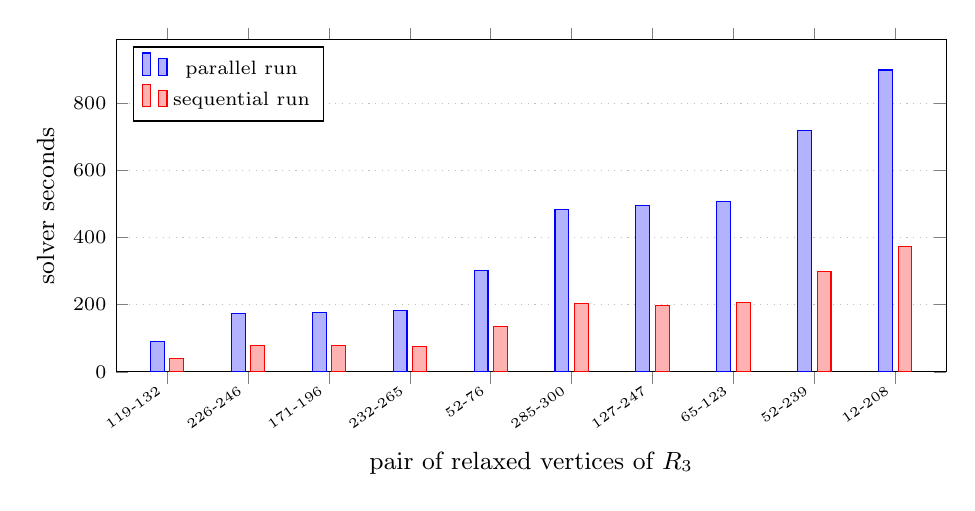
\begin{tikzpicture}
\begin{axis}[ybar,width=\textwidth,height=5.8cm,bar width=5pt,ymin=0,symbolic x coords={119-132,226-246,171-196,232-265,52-76,285-300,127-247,65-123,52-239,12-208},xtick=data,x tick label style={font=\tiny,rotate=35,anchor=east},tick label style={font=\scriptsize},label style={font=\small},ylabel={solver seconds},xlabel={pair of relaxed vertices of $R_3$},legend style={font=\scriptsize,at={(0.02,0.98)},anchor=north west},enlarge x limits=0.07,ymajorgrids=true,grid style={dotted}]
\addplot coordinates {(119-132,91.499) (226-246,173.122) (171-196,177.801) (232-265,182.078) (52-76,302.648) (285-300,483.377) (127-247,495.212) (65-123,507.082) (52-239,718.858) (12-208,898.734)};
\addplot coordinates {(119-132,40.93) (226-246,77.393) (171-196,79.052) (232-265,74.447) (52-76,134.833) (285-300,203.211) (127-247,196.908) (65-123,206.074) (52-239,298.943) (12-208,372.266)};
\legend{parallel run,sequential run}
\end{axis}
\end{tikzpicture}
